Similiar to that in (c), we may obtian the SIR for each signal under $N_r = 64$ received antenna.
The SIR of each signal is listed in the table below:
\begin{table}[H]
    \centering
    \begin{tabular}{c|c|c|c|c|c}
        & Signal 1 & Signal 2 & Signal 3 & Signal 4 & Signal 5 \\  
             \hline 
    SIR (dB) & 21.2980  & 16.7495  & 23.8789  & 21.1201  & 16.7325  
    \end{tabular}
\end{table}
Compared to that in problem 3, it can be observed that the SIR for 
each signal increases as the number of receiving antennas increases.
The reason can be seen from the radiation patterns
\begin{figure}[H]
    \centering
    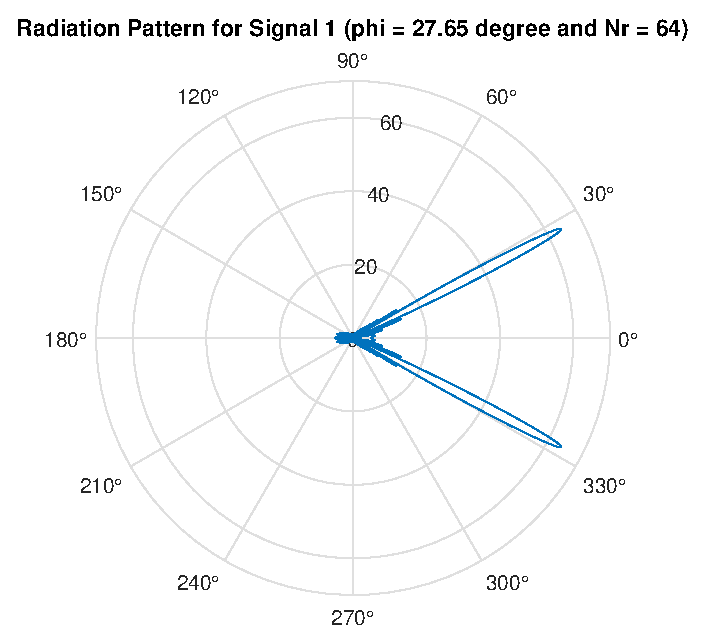
\includegraphics[scale = 0.7]{N64_1.eps}
\end{figure}
\begin{figure}[H]
    \centering
    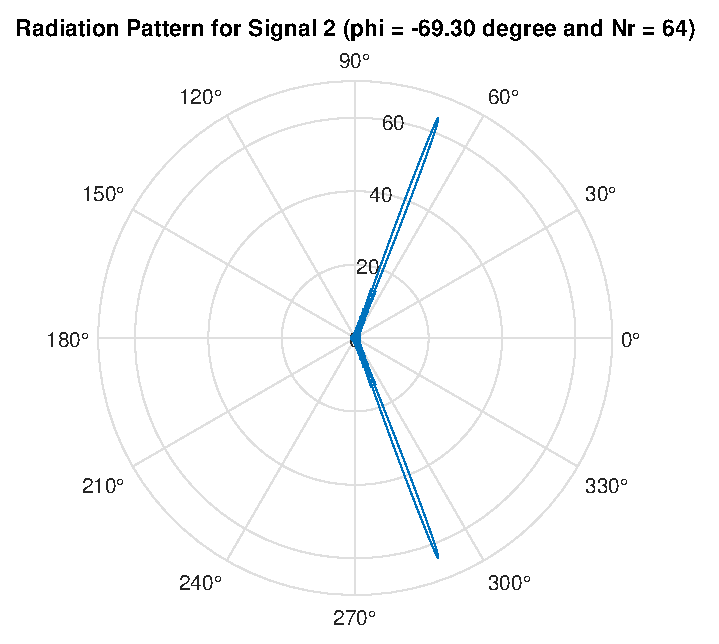
\includegraphics[scale = 0.7]{N64_2.eps}
\end{figure}
\begin{figure}[H]
    \centering
    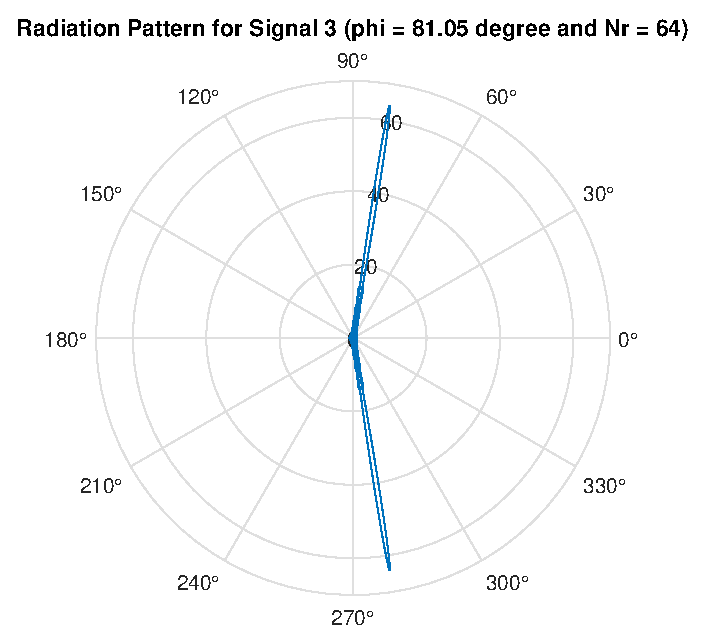
\includegraphics[scale = 0.7]{N64_3.eps}
\end{figure}
\begin{figure}[H]
    \centering
    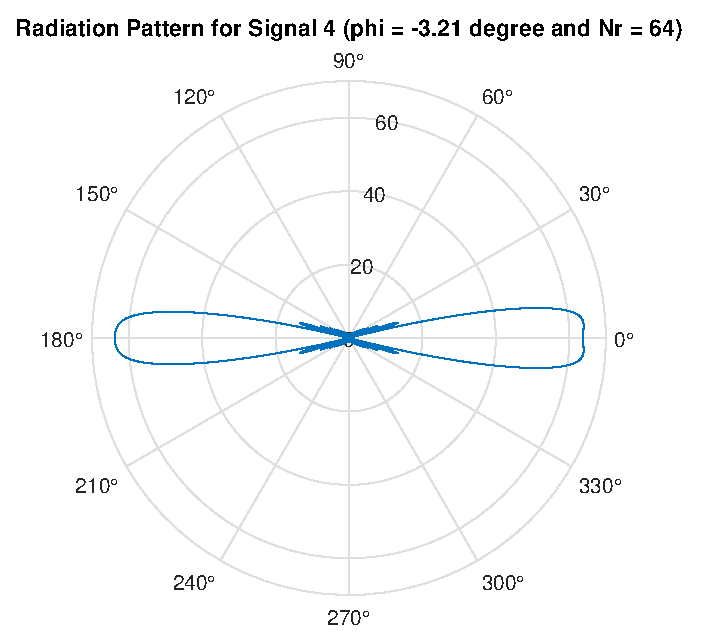
\includegraphics[scale = 0.7]{N64_4.eps}
\end{figure}
\begin{figure}[H]
    \centering
    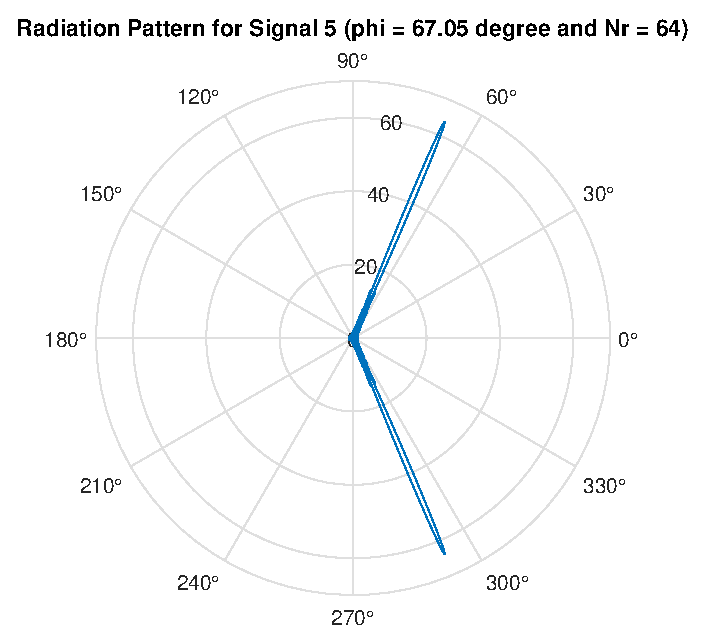
\includegraphics[scale = 0.7]{N64_5.eps}
\end{figure}
It can be seen that as $N_r$ increases, the beamwidth becomes narrower. Hence, the gain at 
angles other than the incidence angle becomes smaller, improving the angular resolvability. 
This also explains why the SIR of signals 2 and 5 is no longer 1.